% =============================================================
%  MechanicPro --- Technical Report
%  Template: Professional / Modern / Clean
% =============================================================

\documentclass[12pt, a4paper]{report}

% -- Encoding & Font ------------------------------------------
\usepackage[T1]{fontenc}
\usepackage[utf8]{inputenc}
\usepackage[scaled=0.92]{helvet}
\renewcommand{\familydefault}{\sfdefault}

\usepackage{float}
\usepackage{xurl}
\usepackage{seqsplit}

% -- Page Layout ----------------------------------------------
\usepackage[
top=2.5cm, bottom=2.5cm,
left=3cm,  right=2.5cm
]{geometry}
% Automatic "Month Year" date (no extra package needed)
\newcommand{\monthyear}{%
	\ifcase\month\or January\or February\or March\or April\or May\or June\or
	July\or August\or September\or October\or November\or December\fi
	\space\the\year%
}
\usepackage{parskip}

% -- Math ---------------------------------------------------
\usepackage{amsmath}

% -- Colors ---------------------------------------------------
\usepackage{xcolor}
\definecolor{Navy}{RGB}{15, 40, 75}
\definecolor{Blue}{RGB}{37, 99, 195}
\definecolor{LightBlue}{RGB}{219, 234, 254}
\definecolor{TextGray}{RGB}{90, 105, 120}
\definecolor{LightGray}{RGB}{248, 249, 251}
\definecolor{RuleGray}{RGB}{220, 225, 232}
\definecolor{StatusGreen}{RGB}{22, 163, 74}

% -- Graphics & Drawing ---------------------------------------
\usepackage{graphicx}
\usepackage{scalerel}
\usepackage{tikz}
\usetikzlibrary{calc}

% -- Tables ---------------------------------------------------
\usepackage{booktabs}
\usepackage{tabularx}
\usepackage{array}
\usepackage{longtable}

% -- Lists ----------------------------------------------------
\usepackage{enumitem}
\setlist[itemize]{leftmargin=1.5em, itemsep=2pt}
\setlist[enumerate]{leftmargin=1.5em, itemsep=2pt}

% -- Code Listings --------------------------------------------
\usepackage{listings}
\lstset{
	basicstyle=\small\ttfamily,
	keywordstyle=\color{Blue}\bfseries,
	commentstyle=\color{TextGray}\itshape,
	stringstyle=\color{StatusGreen},
	backgroundcolor=\color{LightGray},
	frame=single,
	framerule=0pt,
	rulecolor=\color{RuleGray},
	numbers=left,
	numberstyle=\tiny\color{TextGray},
	numbersep=8pt,
	breaklines=true,
	showstringspaces=false,
	tabsize=2,
	xleftmargin=12pt,
}

% -- Headers & Footers ----------------------------------------
\usepackage{fancyhdr}
\pagestyle{fancy}
\fancyhf{}
\fancyhead[L]{%
	\small\color{TextGray}\textit{MechanicPro \textemdash{} Technical Report}%
}
\fancyhead[R]{%
	\small\color{TextGray}v1.0.0%
}
\fancyfoot[L]{%
	\small\color{TextGray}Technical Report%
}
\fancyfoot[R]{%
	\small\color{TextGray}\thepage%
}
\renewcommand{\headrulewidth}{0.4pt}
\renewcommand{\footrulewidth}{0.4pt}
\renewcommand{\headrule}{%
	\color{RuleGray}\hrule width\headwidth height\headrulewidth%
}
\renewcommand{\footrule}{%
	\color{RuleGray}\hrule width\headwidth height\footrulewidth%
}

% Plain style for chapter-opening pages
\fancypagestyle{plain}{%
	\fancyhf{}
	\fancyfoot[R]{\small\color{TextGray}\thepage}
	\renewcommand{\headrulewidth}{0pt}
	\renewcommand{\footrulewidth}{0.4pt}
	\renewcommand{\footrule}{%
		\color{RuleGray}\hrule width\headwidth height\footrulewidth%
	}
}

% -- Section Formatting ---------------------------------------
\usepackage{titlesec}

\titleformat{\chapter}[block]
{\normalfont\huge\bfseries\color{Navy}}
{\color{Blue}\thechapter}{1em}{}
[\vspace{4pt}\color{Blue}\rule{\textwidth}{1.5pt}\vspace{-6pt}]

\titlespacing{\chapter}{0pt}{0pt}{20pt}

\titleformat{\section}
{\normalfont\Large\bfseries\color{Navy}}
{\color{Blue}\thesection}{1em}{}

\titleformat{\subsection}
{\normalfont\large\bfseries\color{TextGray}}
{\thesubsection}{1em}{}

\titleformat{\subsubsection}
{\normalfont\normalsize\bfseries\color{TextGray}}
{\thesubsubsection}{1em}{}

% -- TOC Styling ----------------------------------------------
\usepackage{tocloft}
\renewcommand{\cftchapfont}{\bfseries\color{Navy}}
\renewcommand{\cftchappagefont}{\bfseries\color{Navy}}
\renewcommand{\cftsecfont}{\color{TextGray}}
\renewcommand{\cftsecpagefont}{\color{TextGray}}
\setlength{\cftbeforechapskip}{6pt}

% -- Hyperlinks -----------------------------------------------
\usepackage{hyperref}
\hypersetup{
	colorlinks  = true,
	linkcolor   = Blue,
	urlcolor    = Blue,
	citecolor   = Blue,
	pdftitle    = {MechanicPro --- Technical Report},
	pdfauthor   = {Your Name},
	pdfsubject  = {Technical Report},
	pdfkeywords = {Tauri, React, TypeScript, SQLite, Desktop Application},
}

% -- Custom Commands ------------------------------------------

% Info box
\newcommand{\infobox}[1]{%
	\vspace{6pt}
	\noindent
	\colorbox{LightBlue}{%
		\begin{minipage}{\dimexpr\linewidth-2\fboxsep}%
			\vspace{4pt}
			\small #1
			\vspace{4pt}
		\end{minipage}%
	}
	\vspace{6pt}
}

% Term definition
\newcommand{\term}[1]{\textbf{\color{Blue}#1}}

% Abstract page
\newcommand{\abstractpage}[1]{%
	\clearpage
	\thispagestyle{plain}
	\vspace*{2cm}
	\begin{center}
		{\color{Navy}\Large\bfseries Abstract}\\[0.4cm]
		\color{Blue}\rule{0.3\textwidth}{1.5pt}
	\end{center}
	\vspace{0.8cm}
	\begin{quote}
		\setlength{\parskip}{6pt}
		\normalsize #1
	\end{quote}
	\vfill
	\noindent\small\color{TextGray}
	\textbf{Keywords:} Tauri, React, TypeScript, SQLite, Desktop Application,
	Mechanic Shop Management.
	\clearpage
}
\newcommand{\coverpage}{%
	\begin{titlepage}
		\begin{tikzpicture}[remember picture, overlay]
			
			%% Top bar
			\fill[Navy]
			(current page.north west)
			rectangle
			([yshift=-4cm] current page.north east);
			
			%% Accent stripe below top bar
			\fill[Blue]
			([yshift=-4cm] current page.north west)
			rectangle
			([yshift=-4.12cm] current page.north east);
			
			%% Bottom band
			\fill[LightGray]
			(current page.south west)
			rectangle
			([yshift=3.2cm] current page.south east);
			
			%% Bottom band top border
			\fill[RuleGray]
			([yshift=3.2cm] current page.south west)
			rectangle
			([yshift=3.24cm] current page.south east);
			
		\end{tikzpicture}
		
		%% -- Top bar content ----------------------
		\vspace*{1.2cm}
		\hspace{1.2cm}
		\begin{minipage}{0.8\textwidth}
			{\color{white}\footnotesize\bfseries\MakeUppercase{Technical Report}}
			\quad
			{\color{Blue!40!white}\footnotesize Technical Report}
		\end{minipage}
		
		\vspace{3.6cm}
		
		%% -- Main title block ---------------------
		\hspace{1.2cm}
		\begin{minipage}{0.82\textwidth}
			
			{\color{Navy}\Huge\bfseries\scalebox{2.0}{MechanicPro}}
			
			\vspace{0.3cm}
			{\color{TextGray}\large Management System for a Mechanic Shop}
			
			\vspace{0.6cm}
			\color{Blue}\rule{\textwidth}{1.5pt}
			\vspace{0.3cm}
			
			{\color{TextGray}\normalsize
				System Architecture, Database Design, and Technical Overview
			}
			
		\end{minipage}
		
		\vfill
		
		%% -- Metadata block -----------------------
		\hspace{1.2cm}
		\begin{minipage}{0.82\textwidth}
			\renewcommand{\arraystretch}{1.5}
			\begin{tabular}{>{\color{TextGray}\small\bfseries}l
					>{\small}l
					@{\hskip 2cm}
					>{\color{TextGray}\small\bfseries}l
					>{\small}l}
				Author    & Eduardo Freitas Fernandes      & Version   & 1.0.0      \\
				Date      & \monthyear     & Status    &
				\textcolor{StatusGreen}{\bfseries Final}        \\
				Document  & Technical Report & Language  & English    \\
			\end{tabular}
		\end{minipage}
		
		\vspace{2.8cm}
		
	\end{titlepage}
}

% =============================================================
%  DOCUMENT
% =============================================================

\begin{document}
	
	\coverpage
	
	\abstractpage{%
		This document is the technical report for \textbf{MechanicPro}, a desktop
		application designed to manage the day-to-day operations of a mechanic shop.
		The report describes the system architecture, the technology stack, the
		database design, and the build and release process.
		
		MechanicPro is built with \term{Tauri v2} and \term{Rust} for the desktop
		shell, \term{React 19} and \term{TypeScript} for the user interface, and
		\term{SQLite} for local data persistence. The application runs entirely
		offline, with no server or cloud dependency.
		
		The intended reader is a developer who wants to understand, maintain, or
		extend the system. Usage instructions are covered separately in the User
		Manual.
	}
	
	% -- Revision History -----------------------------------------
	\chapter*{Revision History}
	
	\noindent \begin{tabularx}{\textwidth}{c l X l}
		\toprule
		\textbf{Version} & \textbf{Date} & \textbf{Description} & \textbf{Author} \\
		\midrule
		1.0.0 & June 2026 & Initial document created           & Eduardo Fernandes \\
		\bottomrule
	\end{tabularx}
	
	\vspace{1cm}
	\noindent\small\color{TextGray}
	This document describes version 1.0.0 of MechanicPro.
	For changes to the application itself, refer to the project \texttt{CHANGELOG.md}.
	
	\newpage
	
	% -- Table of Contents ----------------------------------------
	\tableofcontents
	
	\newpage
	
	\listoffigures
	
	\newpage
	
	\listoftables   % uncomment if you add tables
	
	% =============================================================
	%  CHAPTER 1 --- INTRODUCTION
	% =============================================================
	\chapter{Introduction}
	
	\section{Purpose}
	This document is the technical reference for \textbf{MechanicPro} version 1.0.0.
	Its purpose is to describe the internal design of the system in sufficient detail
	that a developer can understand, maintain, or extend the application without
	prior knowledge of the codebase.
	
	The report covers the system architecture, the technology stack, the database
	schema, the state management strategy, and the build and release process.
	It does \emph{not} cover end-user workflows or feature usage; those topics
	are addressed separately in the User Manual.
	
	\section{Scope}
	This document applies exclusively to the \textbf{desktop application} component
	of MechanicPro. The following topics are in scope:
	
	\begin{itemize}
		\item Overall system architecture and the two-process model (WebView + Tauri shell).
		\item Frontend structure: pages, components, routing, and state management.
		\item Backend integration: the Tauri SQL plugin and the service layer.
		\item Database design: schema, relationships, business rules, and soft-delete strategy.
		\item CSV import and export format specification.
		\item Development environment setup, production build process, and output artefacts.
		\item Known technical limitations of the current release.
	\end{itemize}
	
	The following topics are explicitly \textbf{out of scope}: user interface usage
	instructions, network infrastructure (the application has none), and future
	roadmap items.
	
	\section{Intended Audience}
	This document is intended for \textbf{developers} who need to work with the
	MechanicPro codebase. The reader is assumed to have working knowledge of:
	
	\begin{itemize}
		\item TypeScript and the React component model.
		\item Relational database concepts (tables, primary keys, foreign keys).
		\item Basic command-line usage (running \texttt{npm} and \texttt{cargo} commands).
	\end{itemize}
	
	No prior knowledge of Tauri or Rust is required to understand the frontend
	sections of this report. The backend sections that touch on Tauri configuration
	are self-contained and include sufficient context.
	
	\section{Document Conventions}
	The following conventions are used throughout this report:
	
	\begin{itemize}
		\item \textbf{Bold text} is used to introduce key terms or to emphasise
		      important statements.
		\item \term{Coloured bold text} (e.g., \term{Zustand}) denotes a named
		      technology, library, or architectural concept.
		\item \texttt{Monospace text} is used for file names, directory paths,
		      command-line instructions, and inline code references.
		\item Code blocks with line numbers are used for multi-line source code
		      and shell commands.
		\item Blue information boxes are used to call attention to notable
		      constraints, warnings, or design decisions.
	\end{itemize}
	
	\infobox{\textbf{Note:} Blue boxes like this one highlight important
		information or design decisions that deserve special attention.}
	
	% =============================================================
	%  CHAPTER 2 --- SYSTEM OVERVIEW
	% =============================================================
	\chapter{System Overview}
	
	\section{Application Purpose}
	\textbf{MechanicPro} is a desktop application designed to manage the
	day-to-day operations of a small mechanic shop. It provides a centralised,
	offline system for recording and querying:

	\begin{itemize}
		\item \textbf{Clients} --- the vehicle owners who bring their cars for service.
		\item \textbf{Vehicles} --- each registered car, associated with one client.
		\item \textbf{Service Orders} --- repair and maintenance records linked to a
		      vehicle, including itemised operations, mileage, labour hours, and total price.
	\end{itemize}

	The application also provides a \textbf{Dashboard} with summary statistics and
	trend charts, and supports \textbf{CSV import and export} to allow data migration
	and backup. Service orders can be printed or downloaded as a \textbf{PDF invoice}.

	MechanicPro runs entirely \textbf{offline}. It has no server, no cloud dependency,
	and no network requirement at runtime. All data is stored locally in a single
	SQLite database file on the user's machine.

	\section{Technology Stack}

	Table~\ref{tab:stack} lists the libraries and frameworks that make up the
	MechanicPro technology stack.

	\begin{table}[H]
		\centering
		\begin{tabularx}{\textwidth}{l l X}
			\toprule
			\textbf{Layer}    & \textbf{Technology}              & \textbf{Role} \\
			\midrule
			UI Framework      & React 19 + TypeScript            & Component-based frontend interface \\
			Build Tool        & Vite 7                           & Development server and production bundler \\
			Desktop Shell     & Tauri v2 (Rust)                  & Native window, OS integration, and IPC bridge \\
			Database          & SQLite via \texttt{plugin-sql}   & Local, file-based data persistence \\
			State Management  & Zustand 5                        & Global client-side state and mutation orchestration \\
			Routing           & react-router-dom v7              & Client-side page navigation \\
			Charts            & recharts                         & Dashboard statistics visualisations \\
			PDF Generation    & jsPDF + html2canvas              & Service order invoice export \\
			Icons             & lucide-react                     & Consistent UI icon set \\
			\bottomrule
		\end{tabularx}
		\caption{MechanicPro technology stack}
		\label{tab:stack}
	\end{table}

	\section{System Requirements}

	\subsection*{Runtime Requirements}
	\begin{itemize}
		\item \textbf{Windows 10 / 11} (x64): Microsoft \term{WebView2} runtime must
		      be installed. It is bundled automatically in the distributed installer.
		\item \textbf{macOS 10.15 Catalina or later}: Uses the system \term{WKWebView}.
		      No additional runtime is required.
		\item \textbf{Linux} (x64): A compatible \term{WebKitGTK} installation is
		      required (typically available by default on modern desktop distributions).
	\end{itemize}

	\subsection*{Hardware Requirements}
	MechanicPro has no demanding hardware requirements. Any machine capable of running
	a modern web browser is sufficient. Approximate minimum specifications:

	\begin{itemize}
		\item \textbf{RAM}: 256 MB available (the application is lightweight).
		\item \textbf{Disk}: 50 MB for the installer; additional space for the SQLite
		      database, which grows proportionally to the volume of records.
		\item \textbf{Display}: 1024 × 768 minimum resolution. The UI is optimised
		      for 1280 × 800 and above.
	\end{itemize}

	\subsection*{Development Prerequisites}
	Building from source additionally requires:
	\begin{itemize}
		\item \textbf{Node.js} 18 or later (with \texttt{npm}).
		\item \textbf{Rust} stable toolchain (via \texttt{rustup}).
		\item Platform-specific Tauri build dependencies as documented at
		      \url{https://tauri.app/start/prerequisites/}.
	\end{itemize}

	\section{High-Level Data Flow}

	All data access in MechanicPro follows a strict, layered path from the UI
	down to the SQLite database and back. Figure~\ref{fig:dataflow} illustrates
	this flow at a high level.

	\begin{enumerate}
		\item \textbf{User Interaction}: The user performs an action in the React UI
		      (e.g., clicks ``Save'' on a new client form).
		\item \textbf{Zustand Store}: The UI calls an action on the relevant
		      \term{Zustand} store (e.g., \texttt{useClientStore. createClient()}).
		      The store sets a \texttt{loading} flag and delegates to the service layer.
		\item \textbf{Service Layer}: A TypeScript service module (e.g.,
		      \texttt{clientService.ts}) constructs the SQL query and calls
		      \texttt{db.execute()} or \texttt{db.select()}.
		\item \textbf{Tauri SQL Plugin}: The \texttt{@tauri-apps/plugin-sql} library
		      serialises the query and parameters as JSON and sends them over the
		      \term{IPC} bridge to the Tauri Rust core.
		\item \textbf{Rust Core / SQLite}: The Rust side of the plugin executes the
		      query against the local SQLite file (\texttt{mechanicpro.db}) and returns
		      the result as a JSON payload.
		\item \textbf{Store Update}: The Zustand store receives the result, updates
		      its state (e.g., the \texttt{clients} array), and clears the
		      \texttt{loading} flag. React re-renders only the components that
		      subscribe to the changed state slice.
	\end{enumerate}

	\begin{figure}[H]
		\centering
		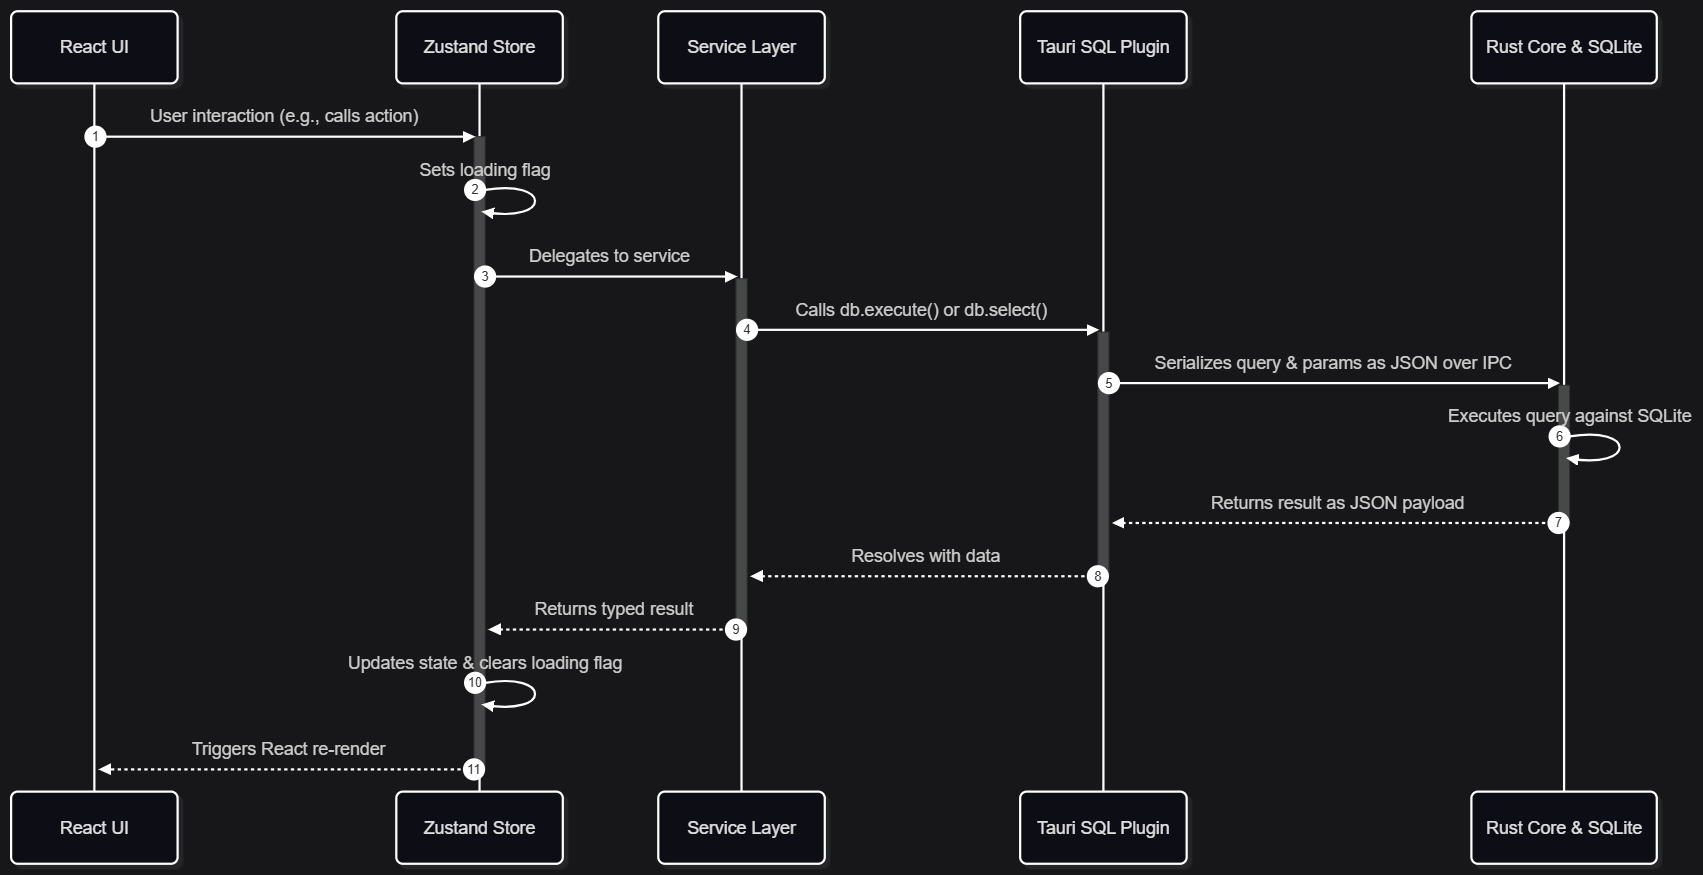
\includegraphics[width=0.9\textwidth]{figures/dataflow.png}
		\caption{High-level data flow from user interaction to SQLite and back}
		\label{fig:dataflow}
	\end{figure}

	\infobox{\textbf{Note:} There are no custom Rust commands in MechanicPro. All
		database access is handled entirely from the TypeScript side using the
		\term{Tauri SQL plugin's} JavaScript bindings. The Rust layer is used
		solely for its native window, OS integration, and IPC capabilities.}
	
	% =============================================================
	%  CHAPTER 3 --- ARCHITECTURE
	% =============================================================
	\chapter{Architecture}

	\section{Overview}
	MechanicPro follows the \term{Tauri two-process model}. The application is
	composed of two isolated processes that communicate exclusively through a
	structured IPC bridge:

	\begin{itemize}
		\item \textbf{The WebView process} --- a Chromium-based (Windows) or
		      WebKit-based (macOS/Linux) renderer that runs the React + TypeScript
		      frontend. This process has no direct access to the filesystem,
		      operating system APIs, or the SQLite file.
		\item \textbf{The Rust core process} --- the native Tauri host process,
		      compiled from Rust. It owns the application window, manages OS
		      permissions, and hosts the plugin runtime that has privileged access
		      to system resources including the SQLite database.
	\end{itemize}

	The two processes cannot share memory. All data exchange between the frontend
	and the Rust core is serialised to JSON and passed through Tauri's
	\term{IPC bridge}. In MechanicPro, this bridge is used exclusively by the
	\texttt{@tauri-apps/plugin-sql} library --- there are no hand-authored Tauri
	commands or Rust source files in the project beyond the default Tauri scaffold.

	\section{Frontend - React and TypeScript}

	\subsection{Component Structure}
	The frontend source lives in \texttt{app/src/} and is divided into four
	categories:

	\begin{itemize}
		\item \textbf{Pages} (\texttt{src/pages/}): Route-level components, each
		      corresponding to a distinct view in the application. There are eight
		      pages in total (see Section~\ref{sec:routing}).
		\item \textbf{Components} (\texttt{src/components/}): Reusable UI elements
		      shared across pages. These include modal dialogs and structural
		      components.
		\item \textbf{Stores} (\texttt{src/store/}): Zustand global state modules
		      (see Section~\ref{sec:state}).
		\item \textbf{Services} (\texttt{src/services/}): TypeScript modules that
		      encapsulate all SQL queries and business logic (see
		      Section~\ref{sec:ipc}).
	\end{itemize}

	Table~\ref{tab:components} lists the components in \texttt{src/components/}
	and their roles.

	\begin{table}[H]
		\centering
		\begin{tabularx}{\textwidth}{l X}
			\toprule
			\textbf{Component}            & \textbf{Role} \\
			\midrule
			\texttt{Layout.tsx}           & Root shell; renders the sidebar and the \texttt{<Outlet />} for nested routes \\
			\texttt{Sidebar.tsx}          & Navigation menu with links to all pages \\
			\texttt{ClientModal.tsx}      & Modal form for creating and editing clients \\
			\texttt{VehicleModal.tsx}     & Modal form for creating and editing vehicles \\
			\texttt{ConfirmModal.tsx}     & Generic confirmation dialog for destructive actions \\
			\texttt{VehicleHistoryOverlay.tsx} & Slide-in panel displaying the full service history for a vehicle \\
			\texttt{PrintTemplate.tsx}    & Hidden DOM element used by html2canvas for PDF generation \\
			\bottomrule
		\end{tabularx}
		\caption{Reusable components in \texttt{src/components/}}
		\label{tab:components}
	\end{table}

	\subsection{State Management}
	\label{sec:state}
	Global application state is managed with \term{Zustand} (v5). Three stores
	are defined in \texttt{src/store/}, one per primary entity domain:

	\begin{itemize}
		\item \texttt{useClientStore.ts} --- holds the \texttt{clients} array,
		      the active \texttt{search} string, and async mutation actions
		      (\texttt{createClient}, \texttt{updateClient}, \texttt{deleteClient}).
		\item \texttt{useVehicleStore.ts} --- holds the \texttt{vehicles} array,
		      the active \texttt{search} string, and the equivalent mutation actions.
		\item \texttt{useServiceOrderStore.ts} --- holds the \texttt{serviceOrders}
		      array, the active \texttt{search} string, the \texttt{sortOrder}
		      preference (\texttt{ASC}/\texttt{DESC}), and mutation actions.
	\end{itemize}

	Each store follows the same pattern: every mutation action (\texttt{create},
	\texttt{update}, \texttt{delete}) calls the corresponding service function,
	then automatically calls \texttt{fetchX()} to refresh the list. This ensures
	that all components subscribed to the store see the updated data without
	requiring manual callback chains or prop drilling.

	Search terms and sort preferences are persisted to \texttt{sessionStorage} so
	that navigation between pages does not reset the user's last query.

	\infobox{\textbf{Design Note:} Zustand stores act as both the state container
		and the hook interface. Components call \texttt{useClientStore()} directly;
		no additional custom hook wrapper layer is needed.}

	\subsection{Routing}
	\label{sec:routing}
	Client-side routing is handled by \term{react-router-dom} v7. The route
	tree is defined in \texttt{src/App.tsx} using a single nested layout route:

	\begin{table}[H]
		\centering
		\begin{tabularx}{\textwidth}{l l X}
			\toprule
			\textbf{Path}           & \textbf{Component}              & \textbf{Description} \\
			\midrule
			\texttt{/}              & \texttt{DashboardPage}          & Summary statistics and trend charts \\
			\texttt{/clients}       & \texttt{ClientsPage}            & Searchable client list with CRUD \\
			\texttt{/vehicles}      & \texttt{VehiclesPage}           & Searchable vehicle list with CRUD \\
			\texttt{/services}      & \texttt{ServicesPage}           & Service order list with search and sort \\
			\texttt{/services/new}  & \texttt{CreateServiceOrderPage} & Multi-step form to create a service order \\
			\texttt{/services/:id}  & \texttt{ServiceOrderDetailsPage}& Detail view, print, and PDF export \\
			\texttt{/import}        & \texttt{ImportPage}             & CSV data import for all three entities \\
			\texttt{/export}        & \texttt{ExportPage}             & CSV data export for all three entities \\
			\bottomrule
		\end{tabularx}
		\caption{Application routes}
		\label{tab:routes}
	\end{table}

	All routes are rendered inside the \texttt{Layout} component, which provides
	the persistent sidebar navigation. There is no lazy loading; all page
	components are bundled into a single chunk.

	\section{Backend - Tauri and Rust}

	\subsection{Tauri Commands}
	MechanicPro does \textbf{not} define any custom Tauri commands. The default
	Tauri scaffold generates a minimal \texttt{src-tauri/src/main.rs} that
	registers the application and the required plugins. No additional
	\texttt{\#[tauri::command]} functions have been authored.

	All privileged operations (database access) are delegated to the
	\texttt{plugin-sql} plugin, which exposes its own pre-built command surface
	over the IPC bridge.

	\subsection{Plugin Usage}
	A single Tauri plugin is used in production:

	\begin{itemize}
		\item \textbf{\texttt{@tauri-apps/plugin-sql}} (JS) /
		      \textbf{\texttt{tauri-plugin-sql}} (Rust): Provides \texttt{db.execute()}
		      and \texttt{db.select()} methods in the TypeScript layer, which are
		      transmitted over IPC to the Rust side and executed against a local
		      SQLite file. The plugin is declared in \texttt{tauri.conf.json} under
		      the \texttt{plugins.sql} key and initialised on first call to
		      \texttt{Database.load("sqlite:mechanicpro.db")}.
	\end{itemize}

	\section{IPC Communication}
	\label{sec:ipc}
	The \term{IPC bridge} in Tauri transmits messages as JSON over a local
	channel between the WebView and the Rust process. In MechanicPro, IPC
	calls are never made directly by application code. Instead, all IPC
	is mediated through the service layer:

	\begin{enumerate}
		\item A service function calls \texttt{db.execute(sql, params)} or
		      \texttt{db.select<T[]>(sql, params)}.
		\item The plugin serialises the query string and the parameter array
		      to JSON and dispatches a Tauri \texttt{invoke()} call internally.
		\item The Rust plugin handler deserialises the payload, binds the
		      parameters, executes the query, and serialises the row results back
		      to JSON.
		\item The TypeScript \texttt{Promise} resolves with the typed result.
	\end{enumerate}

	SQL parameters are always passed as a positional array (using \texttt{?}
	placeholders), which prevents SQL injection. Errors thrown on the Rust side
	are propagated as rejected \texttt{Promise}s and caught by the calling store
	action, which stores the error message in its \texttt{error} state field.

	\section{Folder Structure}
	The annotated repository layout is shown in Listing~\ref{lst:tree}.

	\begin{lstlisting}[language=bash, caption={Repository structure}, label={lst:tree}]
MechanicPro/
+--- app/                        # Vite + React + Tauri frontend project
|   +--- src/
|   |   +--- components/       # Reusable UI components
|   |   +--- pages/            # Route-level page components
|   |   +--- services/         # SQL query and business logic modules
|   |   +--- store/            # Zustand global state stores
|   |   +--- db.ts             # DB singleton, table init, TypeScript interfaces
|   |   +--- App.tsx           # Router definition
|   |   +--- App.css           # Global design system styles
|   |   `--- main.tsx          # React entry point
|   +--- src-tauri/
|   |   +--- src/
|   |   |   `--- main.rs       # Tauri app entry point and plugin registration
|   |   +--- Cargo.toml        # Rust dependencies
|   |   `--- tauri.conf.json   # Tauri configuration (app name, version, plugins)
|   +--- package.json
|   `--- vite.config.ts
+--- docs/                     # Technical documentation
|   +--- figures/              # Images referenced in the report
|   `--- TechnicalReport.tex   # This document
+--- CHANGELOG.md
`--- README.md
	\end{lstlisting}


	% =============================================================
	%  CHAPTER 4 --- DATABASE
	% =============================================================
	\chapter{Database}

	\section{Overview}
	MechanicPro uses \term{SQLite} as its sole data store. The database is a
	single file named \texttt{mechanicpro.db}, managed by the
	\texttt{tauri-plugin-sql} Rust plugin. The file is created automatically
	on first launch and stored in the platform's standard application data
	directory:

	\begin{itemize}
		\item \textbf{Windows}: \texttt{\%APPDATA\%\textbackslash{}MechanicPro\textbackslash{}mechanicpro.db}
		\item \textbf{macOS}: \texttt{\textasciitilde{}/Library/Application Support/MechanicPro/mechanicpro.db}
		\item \textbf{Linux}: \texttt{\textasciitilde{}/.local/share/MechanicPro/mechanicpro.db}
	\end{itemize}

	The schema is initialised idempotently on every application start via
	\texttt{CREATE TABLE IF NOT EXISTS} and \texttt{CREATE UNIQUE INDEX IF NOT EXISTS}
	statements executed in \texttt{src/db.ts}. No migration framework is used;
	the schema is designed to be stable across the v1.0.0 lifecycle.

	\infobox{\textbf{Note:} The SQLite database file is stored in plaintext.
		No encryption at rest is applied in this version. For sensitive
		deployments, filesystem-level encryption should be considered.}

	\section{Schema}
	The database consists of four tables. All tables implement a
	\textbf{soft-delete} pattern: records are never physically removed.
	Instead, a \texttt{deleted\_at} timestamp is set, and all queries
	filter on \texttt{deleted\_at IS NULL} to exclude deleted rows.

	\subsection{\texttt{clients}}
	Stores the vehicle owners registered in the system.

	\begin{table}[H]
		\centering
		\begin{tabularx}{\textwidth}{l l l X}
			\toprule
			\textbf{Column}    & \textbf{Type}   & \textbf{Constraints}   & \textbf{Description} \\
			\midrule
			\texttt{id}         & INTEGER & PK, AUTOINCREMENT      & Unique client identifier \\
			\texttt{name}       & TEXT    & NOT NULL               & Full name of the client \\
			\texttt{phone}      & TEXT    & ---                    & Optional contact phone number \\
			\texttt{created\_at} & DATETIME & DEFAULT CURRENT\_TIMESTAMP & Record creation timestamp \\
			\texttt{deleted\_at} & DATETIME & ---                   & Soft-delete timestamp; NULL means active \\
			\bottomrule
		\end{tabularx}
		\caption{Schema for the \texttt{clients} table}
		\label{tab:clients}
	\end{table}

	A partial unique index on \texttt{name} (where \texttt{deleted\_at IS NULL})
	enforces that no two \emph{active} clients share the same name. Deleted
	records are excluded from the uniqueness constraint, so a name can be
	re-registered after the original record is deleted.

	\subsection{\texttt{vehicles}}
	Stores vehicles, each belonging to exactly one client.

	\begin{table}[H]
		\centering
		\begin{tabularx}{\textwidth}{l l l X}
			\toprule
			\textbf{Column}    & \textbf{Type}   & \textbf{Constraints}   & \textbf{Description} \\
			\midrule
			\texttt{id}         & INTEGER & PK, AUTOINCREMENT      & Unique vehicle identifier \\
			\texttt{client\_id}  & INTEGER & NOT NULL, FK $\rightarrow$ \texttt{clients.id} & Owner of the vehicle \\
			\texttt{plate}      & TEXT    & NOT NULL               & Licence plate in uppercase \\
			\texttt{brand}      & TEXT    & NOT NULL               & Vehicle manufacturer (e.g., Toyota) \\
			\texttt{model}      & TEXT    & NOT NULL               & Vehicle model name \\
			\texttt{year}       & INTEGER & ---                    & Optional model year \\
			\texttt{created\_at} & DATETIME & DEFAULT CURRENT\_TIMESTAMP & Record creation timestamp \\
			\texttt{deleted\_at} & DATETIME & ---                   & Soft-delete timestamp; NULL means active \\
			\bottomrule
		\end{tabularx}
		\caption{Schema for the \texttt{vehicles} table}
		\label{tab:vehicles}
	\end{table}

	A partial unique index on \texttt{plate} (where \texttt{deleted\_at IS NULL})
	prevents duplicate licence plates among active vehicles. Plates are
	normalised to uppercase by the service layer before insertion.

	\subsection{\texttt{service\_orders}}
	The central entity of the application. Each record represents one repair
	or maintenance visit for a vehicle.

	\begin{table}[H]
		\centering
		\begin{tabularx}{\textwidth}{l l l X}
			\toprule
			\textbf{Column}      & \textbf{Type}   & \textbf{Constraints}   & \textbf{Description} \\
			\midrule
			\texttt{id}           & INTEGER & PK, AUTOINCREMENT      & Unique order identifier \\
			\texttt{vehicle\_id}  & INTEGER & NOT NULL, FK $\rightarrow$ \texttt{vehicles.id} & Vehicle serviced \\
			\texttt{mileage}      & INTEGER & NOT NULL               & Vehicle odometer reading at time of service \\
			\texttt{hours}        & REAL    & NOT NULL               & Labour hours worked \\
			\texttt{hourly\_rate}  & REAL    & NOT NULL               & Labour rate per hour \\
			\texttt{observations} & TEXT    & ---                    & Optional free-text notes \\
			\texttt{total\_price}  & REAL    & NOT NULL               & Computed total (labour + operations); stored at insert time \\
			\texttt{created\_at}  & DATETIME & DEFAULT CURRENT\_TIMESTAMP & Date and time of the service order \\
			\texttt{deleted\_at}  & DATETIME & ---                   & Soft-delete timestamp; NULL means active \\
			\bottomrule
		\end{tabularx}
		\caption{Schema for the \texttt{service\_orders} table}
		\label{tab:service_orders}
	\end{table}

	\subsection{\texttt{service\_operations}}
	Stores the individual line items (parts replaced, repairs performed)
	that belong to a service order. There is no soft delete on this table;
	operations are physically deleted when the parent order is soft-deleted
	(cascade is handled at the application layer).

	\begin{table}[H]
		\centering
		\begin{tabularx}{\textwidth}{l l l X}
			\toprule
			\textbf{Column}           & \textbf{Type}   & \textbf{Constraints}   & \textbf{Description} \\
			\midrule
			\texttt{id}                & INTEGER & PK, AUTOINCREMENT      & Unique operation identifier \\
			\texttt{service\_order\_id} & INTEGER & NOT NULL, FK $\rightarrow$ \texttt{service\_orders.id} & Parent service order \\
			\texttt{description}       & TEXT    & NOT NULL               & Description of the operation or part \\
			\texttt{price}             & REAL    & NOT NULL               & Price charged for this line item \\
			\bottomrule
		\end{tabularx}
		\caption{Schema for the \texttt{service\_operations} table}
		\label{tab:operations}
	\end{table}

	\section{Entity-Relationship Diagram}
	Figure~\ref{fig:er} illustrates the relationships between the four tables.

	\begin{figure}[H]
		\centering
		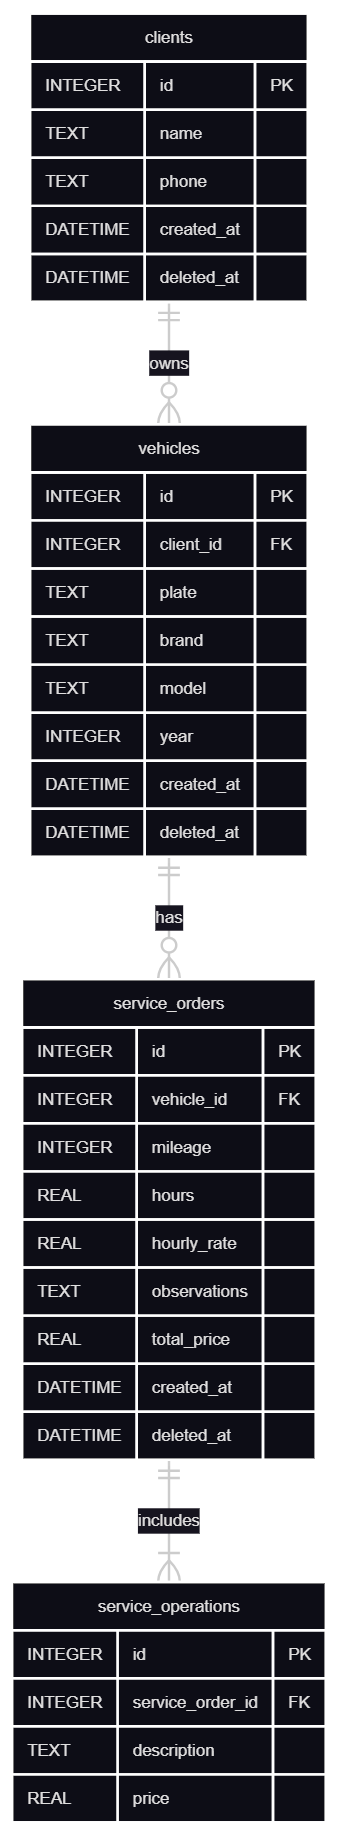
\includegraphics[width=0.15\textwidth]{figures/er_diagram.png}
		\caption{Entity-Relationship Diagram for the MechanicPro database}
		\label{fig:er}
	\end{figure}

	\section{Business Rules}
	The following business rules are enforced at the application and database
	level:

	\begin{itemize}
		\item \textbf{Client name uniqueness}: A partial unique index on
		      \texttt{clients(name) WHERE deleted\_at IS NULL} ensures no two
		      active clients share a name. The check is also performed
		      application-side in \texttt{clientService.ts} to provide a
		      user-friendly error message before the constraint fires.
		\item \textbf{Licence plate uniqueness}: Equivalent partial unique
		      index on \texttt{vehicles(plate) WHERE deleted\_at IS NULL}.
		      Plates are normalised to uppercase before comparison.
		\item \textbf{Total price calculation}: The \texttt{total\_price} of a
		      service order is calculated at insert time as:
		      \[
		        \texttt{total\_price} = (\texttt{hours} \times \texttt{hourly\_rate})
		        + \sum_{\text{operations}} \texttt{price}
		      \]
		      The value is stored in the database and not recalculated on read,
		      ensuring historical records remain accurate even if rates change.
		\item \textbf{Soft deletes}: No \texttt{DELETE} statements are issued
		      against the three main tables. All queries that list data filter
		      on \texttt{deleted\_at IS NULL}.
		\item \textbf{Required fields}: \texttt{clients.name},
		      \texttt{vehicles.client\_id}, \texttt{vehicles.plate},
		      \texttt{vehicles.brand}, \texttt{vehicles.model},
		      \texttt{service\_orders.vehicle\_id}, \texttt{service\_orders.mileage},
		      \texttt{service\_orders.hours}, \texttt{service\_orders.hourly\_rate},
		      and \texttt{service\_operations.description} are all \texttt{NOT NULL}.
	\end{itemize}

	\section{CSV Format}
	All CSV files use \textbf{comma} as the delimiter and \textbf{UTF-8} encoding
	with a BOM (\texttt{U+FEFF}) prepended for Microsoft Excel compatibility.
	Values that contain commas, double quotes, or newlines are wrapped in double
	quotes and internal quotes are escaped as \texttt{""}.

	\subsection*{Clients CSV (\texttt{clientes\_\{date\}.csv})}
	\begin{table}[H]
		\centering
		\begin{tabularx}{\textwidth}{l l X}
			\toprule
			\textbf{Header}         & \textbf{Type}   & \textbf{Notes} \\
			\midrule
			\texttt{ID}             & Integer & Auto-generated database identifier \\
			\texttt{Nome}           & String  & Client name; required on import \\
			\texttt{Telefone}       & String  & Optional; empty string if not set \\
			\texttt{Data de Criação} & String & Date formatted as \texttt{dd/mm/yyyy} (pt-PT locale) \\
			\bottomrule
		\end{tabularx}
		\caption{Clients CSV column specification}
	\end{table}

	\subsection*{Vehicles CSV (\texttt{veiculos\_\{date\}.csv})}
	\begin{table}[H]
		\centering
		\begin{tabularx}{\textwidth}{l l X}
			\toprule
			\textbf{Header}          & \textbf{Type}   & \textbf{Notes} \\
			\midrule
			\texttt{ID}              & Integer & Auto-generated database identifier \\
			\texttt{Matrícula}       & String  & Licence plate in uppercase; required; must be unique \\
			\texttt{Marca}           & String  & Brand name; required \\
			\texttt{Modelo}          & String  & Model name; required \\
			\texttt{Ano}             & Integer & Optional; empty string if not set \\
			\texttt{Cliente}         & String  & Must exactly match an existing active client's name \\
			\texttt{Data de Criação} & String  & Date formatted as \texttt{dd/mm/yyyy} (pt-PT locale) \\
			\bottomrule
		\end{tabularx}
		\caption{Vehicles CSV column specification}
	\end{table}

	\subsection*{Services CSV (\texttt{servicos\_\{date\}.csv})}
	\begin{table}[H]
		\centering
		\begin{tabularx}{\textwidth}{l l X}
			\toprule
			\textbf{Header}          & \textbf{Type}   & \textbf{Notes} \\
			\midrule
			\texttt{ID}              & Integer & Auto-generated database identifier \\
			\texttt{Cliente}         & String  & Client name \\
			\texttt{Matrícula}       & String  & Licence plate; must match an existing active vehicle \\
			\texttt{Quilometragem}   & Integer & Odometer reading in kilometres \\
			\texttt{Horas}           & Decimal & Labour hours worked \\
			\texttt{Preço/Hora}      & Decimal & Hourly labour rate \\
			\texttt{Operações: Preço}& String  & Pipe-separated list of \texttt{description: price} entries \\
			\texttt{Observações}     & String  & Optional free-text notes \\
			\texttt{Data}            & String  & Date formatted as \texttt{dd/mm/yyyy} (pt-PT locale) \\
			\bottomrule
		\end{tabularx}
		\caption{Services CSV column specification}
	\end{table}

	\infobox{\textbf{Import ordering dependency:} CSV files must be imported in
		the following order: \textbf{Clients} first, then \textbf{Vehicles},
		then \textbf{Services}. Each entity references the previous one by name
		or plate, and the import will skip rows where the referenced entity is
		not}
    
    % =============================================================
	%  CHAPTER 5 --- BUILD AND RELEASE
	% =============================================================
	\chapter{Build and Release}

	\section{Development Environment Setup}
	The following prerequisites must be installed before working with the
	MechanicPro source code:

	\begin{itemize}
		\item \textbf{Node.js} 18 or later with \texttt{npm}.
		\item \textbf{Rust} stable toolchain, installed via \texttt{rustup}
		      (\url{https://rustup.rs}).
		\item \textbf{Platform-specific Tauri dependencies} documented at
		      \url{https://tauri.app/start/prerequisites/} (e.g., WebView2 SDK
		      on Windows, \texttt{webkit2gtk} on Linux).
	\end{itemize}

	Once the prerequisites are in place, clone the repository and run the
	following commands from the \texttt{app/} directory:

	\begin{lstlisting}[language=bash, caption={Install dependencies and start the development server}]
cd app
npm install
npm run tauri dev
	\end{lstlisting}

	This starts the Vite development server on \texttt{http://localhost:1420}
	and launches a Tauri window pointed at that URL. Hot module replacement
	(HMR) is active for the React frontend; Rust changes require a full restart.

	\section{Build Process}
	The production build is triggered with a single command from the \texttt{app/}
	directory:

	\begin{lstlisting}[language=bash, caption={Production build command}]
npm run tauri build
	\end{lstlisting}

	This command executes the following pipeline in sequence:

	\begin{enumerate}
		\item \textbf{Frontend build} (\texttt{npm run build}): Vite compiles and
		      bundles all TypeScript and CSS into optimised static assets in
		      \texttt{app/dist/}.
		\item \textbf{Rust compilation} (\texttt{cargo build --release}): The Tauri
		      Rust crate is compiled with the \texttt{release} profile. This step
		      embeds the frontend \texttt{dist/} assets directly into the binary.
		\item \textbf{Packaging}: Tauri wraps the compiled binary into a
		      platform-native installer or bundle according to the
		      \texttt{bundle.targets} setting in \texttt{tauri.conf.json}.
	\end{enumerate}

	\infobox{\textbf{Note:} The first \texttt{tauri build} on a new machine may
		take several minutes as Cargo downloads and compiles all Rust dependencies.
		Subsequent builds are significantly faster due to incremental compilation.}

	\section{Output Artefacts}
	Build outputs are placed in \texttt{app/src-tauri/target/release/bundle/}.
	The artefacts produced depend on the host platform:

	\begin{table}[H]
		\centering
		\begin{tabularx}{\textwidth}{l l X}
			\toprule
			\textbf{Platform} & \textbf{Format}        & \textbf{Notes} \\
			\midrule
			Windows           & \texttt{.msi}           & Windows Installer package; bundles WebView2 runtime \\
			Windows           & \texttt{.exe} (NSIS)    & Alternative standalone installer \\
			macOS             & \texttt{.dmg}           & Disk image containing the \texttt{.app} bundle \\
			macOS             & \texttt{.app}           & macOS application bundle \\
			Linux             & \texttt{.deb}           & Debian/Ubuntu package \\
			Linux             & \texttt{.AppImage}      & Portable, distribution-independent binary \\
			\bottomrule
		\end{tabularx}
		\caption{Build output artefacts by platform}
		\label{tab:artefacts}
	\end{table}

	The \texttt{bundle.targets} key in \texttt{tauri.conf.json} is set to
	\texttt{"all"}, meaning all supported formats for the host platform are
	produced in a single build run.

	\section{Configuration}
	Key application settings are centralised in
	\texttt{app/src-tauri/tauri.conf.json}. Table~\ref{tab:config} documents
	the most relevant fields for a developer maintaining or releasing the
	application.

	\begin{table}[H]
		\centering
		\begin{tabularx}{\textwidth}{l l X}
			\toprule
			\textbf{Key}              & \textbf{Value}              & \textbf{Purpose} \\
			\midrule
			\texttt{productName}      & \texttt{MechanicPro}        & Display name used in installers and window title \\
			\texttt{version}          & \texttt{1.0.0}              & Application version embedded in the installer and About dialog \\
			\texttt{identifier}       & \texttt{com.asus.mechanicpro} & Reverse-domain bundle identifier; used by the OS for app data directories \\
			\texttt{devUrl}           & \texttt{http://localhost:1420} & URL loaded by Tauri during \texttt{tauri dev} \\
			\texttt{frontendDist}     & \texttt{../dist}            & Path to the Vite build output, embedded into the binary \\
			\texttt{windows[0].width} & \texttt{800}                & Initial and minimum window width in pixels \\
			\texttt{windows[0].height}& \texttt{600}                & Initial and minimum window height in pixels \\
			\texttt{windows[0].maximized} & \texttt{true}           & Window launches maximised by default \\
			\texttt{bundle.targets}   & \texttt{"all"}              & Produce all platform-appropriate installer formats \\
			\bottomrule
		\end{tabularx}
		\caption{Key \texttt{tauri.conf.json} settings}
		\label{tab:config}
	\end{table}

	\infobox{\textbf{Release checklist:} Before building a release, ensure that
		(1) \texttt{version} in \texttt{tauri.conf.json} is updated,
		(2) \texttt{version} in \texttt{app/package.json} matches,
		(3) \texttt{CHANGELOG.md} is updated, and
		(4) the build passes \texttt{tsc} without errors.}

	% =============================================================
	%  CHAPTER 6 --- KNOWN LIMITATIONS
	% =============================================================
	\chapter{Known Limitations}

	This chapter documents the known technical limitations of MechanicPro v1.0.0.
	These are not bugs; they are deliberate trade-offs made to keep the
	application simple and maintainable for a single-user, single-machine context.

	\begin{itemize}
		\item \textbf{Single-user only.} The SQLite database file is accessed
		      exclusively by the local application instance. There is no
		      concurrency control, no shared network database, and no
		      multi-user or multi-device support.

		\item \textbf{No data encryption at rest.} The \texttt{mechanicpro.db}
		      file is a standard, unencrypted SQLite file. Any user with access
		      to the filesystem can open it with any SQLite client. For
		      deployments handling sensitive data, filesystem-level encryption
		      (e.g., BitLocker, FileVault) is recommended.

		\item \textbf{No automatic backup mechanism.} The application does not
		      perform automated backups of the database file. The recommended
		      backup strategy is to periodically copy \texttt{mechanicpro.db}
		      to an external location or use the CSV export feature.

		\item \textbf{No authentication or access control.} Any user who can
		      launch the application has full read and write access to all data.
		      There is no login screen, no role-based permissions, and no audit
		      log.

		\item \textbf{No network or cloud synchronisation.} The application is
		      entirely offline. There is no API, no sync engine, and no ability
		      to share data between multiple installations automatically.

		\item \textbf{No database migration framework.} Schema changes between
		      versions require manual migration or a full data re-import. The
		      v1.0.0 schema is designed to be final for this release cycle.

		\item \textbf{PDF generation limitations.} Invoice PDFs are generated
		      using \term{html2canvas} to render an off-screen DOM element.
		      Complex CSS layouts or non-Latin characters may not render
		      correctly in all cases. The output is rasterised, not vector-based.

		\item \textbf{Import does not update existing records.} The CSV import
		      feature is append-only. If a client or vehicle already exists with
		      the same name or plate, the row is silently skipped. There is no
		      ``upsert'' behaviour.
	\end{itemize}

	% =============================================================
	%  APPENDICES
	% =============================================================
	\appendix

	\chapter{Glossary}

	\begin{description}[leftmargin=3cm, style=nextline]
		\item[\term{CRUD}]
		      Create, Read, Update, Delete - the four basic operations on
		      persistent data.
		\item[\term{IPC}]
		      Inter-Process Communication. In Tauri, the mechanism by which the
		      WebView (frontend) sends messages to the Rust core (backend) and
		      receives responses.
		\item[\term{Soft Delete}]
		      A deletion strategy where records are not physically removed from
		      the database. Instead, a \texttt{deleted\_at} timestamp is set.
		      Queries exclude soft-deleted rows by filtering on
		      \texttt{deleted\_at IS NULL}.
		\item[\term{SQLite}]
		      A self-contained, serverless, file-based relational database engine.
		      The entire database is stored in a single \texttt{.db} file on disk.
		\item[\term{Tauri}]
		      A framework for building desktop applications using web technologies
		      (HTML/CSS/JavaScript) for the UI and Rust for the native backend.
		      Version 2 is used in this project.
		\item[\term{TypeScript}]
		      A statically typed superset of JavaScript that compiles to plain
		      JavaScript. Used for the entire MechanicPro frontend.
		\item[\term{WebView}]
		      An embedded browser component that renders web content inside a
		      native application window. Tauri uses the operating system's native
		      WebView (Chromium/WebView2 on Windows, WebKit on macOS/Linux).
		\item[\term{Zustand}]
		      A lightweight, hook-based state management library for React.
		      Stores are plain JavaScript objects with actions; no reducers or
		      action creators are required.
	\end{description}

	\chapter{References}

	\begin{itemize}
		\item Tauri Documentation: \url{https://tauri.app/}
		\item Tauri SQL Plugin: \url{https://github.com/tauri-apps/tauri-plugin-sql}
		\item React Documentation: \url{https://react.dev/}
		\item React Router Documentation: \url{https://reactrouter.com/}
		\item Zustand Documentation: \url{https://zustand.docs.pmnd.rs/}
		\item SQLite Documentation: \url{https://www.sqlite.org/docs.html}
		\item Vite Documentation: \url{https://vite.dev/}
		\item recharts Documentation: \url{https://recharts.org/}
		\item jsPDF Documentation: \url{https://artskydj.github.io/jsPDF/}
	\end{itemize}

\end{document}
